\documentclass{../res/univ-projet}

%Import des packages utilisés pour le document
\usepackage[utf8x]{inputenc}
\usepackage[francais]{babel}
\usepackage[T1]{fontenc}
%\usepackage{array}
%\usepackage{hyperref}
%\usepackage{tabularx, longtable}
%\usepackage[table]{xcolor}
%\usepackage{fancyhdr}
%\usepackage{lastpage}

\definecolor{gris}{rgb}{0.95, 0.95, 0.95}

%Redéfinition des marges
%\addtolength{\hoffset}{-2cm}
%\addtolength{\textwidth}{4cm}
\addtolength{\topmargin}{-1cm}
\addtolength{\textheight}{1cm}
\addtolength{\headsep}{0.8cm} 
\addtolength{\footskip}{-0.2cm}


%Import page de garde et structures pour la gestion de projet
%\usepackage{structures}

%Variables
\logo{../res/logo_univ.png}
\title{Spécification Technique de Besoin}
\author{Ibrahima-Sory \bsc{Barry}, Bertille \bsc{Bouillie}}
\projet{GPG}
\projdesc{Interface Graphique GPG}
\filiere{M1SSI - Conduite de Projet}
\version{0.1}
\relecteur{Olivier \bsc{Thibault}}
\signataire{Magali \bsc{Bardet}}
\date{\today}

\histentry{0.4}{08/12/2014}{Complétion de la section ``Objet`` + ajout des modifications demandées par le client.}
\histentry{0.3}{17/11/2014}{Ajout des modifications demandées par le client.}
\histentry{0.2}{09/11/2014}{Ajout des exigences.}
\histentry{0.1}{31/10/2014}{Version initiale.}

% -- Début du document -- %
\begin{document}

%Page de garde
\maketitle
\newpage
%La table des matières
\tableofcontents
\newpage

\section{Objet}

% Présentation succinte du sujet et hyp de travail.
Le document présent est la spécification technique de besoin d'une étude et implantation d'un outil graphique de gestion de clés PGP.

Le projet sera réalisé par une équipe de sept étudiants du master SSI de Rouen, pour le compte de Madame Magali BARDET responsable de ce même master. 

L'objectif du projet est de réaliser une étude complète d'OpenPGP et du logiciel GnuPG, d'en comprendre le fonctionnement détaillé et de rédiger un rapport illustrant toutes les fonctionnalités.

Il est ensuite demandé de proposer une interface graphique pour GnuPG, accompagnée d'un document d'explications et de recommandations pour l'utilisateur.

Enfin, il est demandé d'effectuer des recherches sur les limites cryptographiques de PGP et de produire un document d'analyse de ces limites. \`{A} l'issue de ces recherches, une implantation de l'attaque sur les KeyID sera à fournir.

\subsection{Besoins opérationnels}
L'interface graphique doit proposer l'accès à un maximum de commandes GPG. Le but étant de pouvoir se passer totalement de la ligne de commande GPG dans un terminal. De plus, elle doit permettre à un utilisateur novice en PGP, mais averti en sécurité, de faire facilement des réglages techniques sur ses clefs ainsi que mettre en place sa toile de confiance et la visualiser graphiquement.

L'interface devra donc être à la fois pédagogique et précise, notamment en ce qui concerne la partie toile de confiance, où le but est de faire comprendre un concept essentiel de PGP.

\subsection{Objectifs techniques}

Les objectifs techniques de l'interface graphique pour GnuPG sont :
\begin{itemize}
 \item la gestion fine des clés : choix de la taille, de l'algorithme de chiffrement symétrique,
 \item la gestion et l'aperçu de la toile de confiance,
 \item le chiffrement et le déchiffrement pour le webmailing,
 \item la visualisation de la ou des lignes de commande GnuPG équivalentes pour chaque action lancée.
\end{itemize}

\subsection{Contraintes et recommandations}

L'application doit fonctionner sur le système d'exploitation GNU/Linux, en particulier sous les environnements KDE et Gnome. Optionnellement, elle pourra être compatible Windows.

\subsection{Résultats attendus}
Les livrables attendus pour ce projet sont :
\begin{itemize}
 \item Un rapport complet sur GnuPG et OpenPGP illustrant toutes les fonctionnalités.
 \item Une interface graphique pour GnuPG.
 \item Un document d'explications et de recommandations à l'utilisation de l'interface graphique.
 \item Un rapport d'étude des limites cryptographiques de PGP.
 \item Une implémentation de l'attaque sur les KeyId telle que celle décrite dans l'article «Surveillance généralisée : aux limites de PGP» du numéro 75 du magazine MISC.
\end{itemize}

\section{Documents applicables et de référence}
% Liste des
% - Références des documents quidefinissent formellement les principes
%   directeurs et le hypothèse de travail prise en compte pour l'établissement de la spécification.
% - Références des documents cités dans la STB au titre d'explication ou de justification.
Différents documents de référence :
\begin{itemize}
\item Définitions du standard OpenPGP \href{http://tools.ietf.org/html/rfc4880}{RFC 4880}
  et \href{http://abcdrfc.free.fr/rfc-vf/pdf/rfc2440.pdf}{RFC 2440}.
\item Le logiciel \href{https://www.gnupg.org/}{GnuPG} (GNU Privacy Guard) implantation Open Source
  de OpenPGP.
\item La \href{https://www.gnupg.org/gph/fr/manual.html#AEN541}{toile de confiance} de GnuPG.
\item Editeurs graphiques existants 
  (\href{http://www.gnupg.org/related_software/frontends.en.html}{KGpg, GPA, Seahorse}).
\item Exemple de visualisation d'une toile de confiance sur le site de 
  \href{https://www.archlinux.org/master-keys/#visualization}{archlinux}.
\end{itemize}



\section{Exigences fonctionnelles}
\subsection{Présentation de la mission du produit logiciel}

\subsubsection{Interface graphique}

\begin{tabular}{|>{\centering}p{1cm}|>{}p{8,5cm}|>{\centering}p{2cm}|>{\centering}p{2cm}|}
  \hline
  \color{white}\cellcolor{blue}\bfseries{Id}&
  \color{white}\cellcolor{blue}\bfseries{Intitulé}&
  \color{white}\cellcolor{blue}\bfseries{Acteur(s)}&
  \color{white}\cellcolor{blue}\bfseries{Priorité}\\
  \cr
  \hline
  EF\_1&
  Exécution d'actions GPG&
  Utilisateur&
  Indispensable
  \cr
  \hline
  EF\_2&
  Chiffrer/déchiffrer/Signer/Vérifier&
  Utilisateur&
  Indispensable
  \cr
  \hline
  EF\_3&
  Affichage des commandes, des retours et des erreurs&
  Utilisateur&
  Indispensable
  \cr
  \hline
  EF\_4&
  Choix du profil utilisateur&
  Utilisateur&
  Indispensable
  \cr
  \hline
  EF\_5&
  Modification de la toile de confiance graphique&
  Utilisateur&
  Important
  \cr
  \hline
\end{tabular}\\

\subsubsection{Calcul d'une seconde pré-image pour une clé donnée}
\begin{tabular}{|>{\centering}p{1cm}|>{}p{8,5cm}|>{\centering}p{2cm}|>{\centering}p{2cm}|}
  \hline
  \color{white}\cellcolor{blue}\bfseries{Id}&
  \color{white}\cellcolor{blue}\bfseries{Intitulé}&
  \color{white}\cellcolor{blue}\bfseries{Acteur(s)}&
  \color{white}\cellcolor{blue}\bfseries{Priorité}\\
  \cr
  \hline
  EF\_6&
  Calcul d'une seconde pré-image pour une clé donnée&
  Utilisateur&
  Indispensable
  \cr
  \hline
\end{tabular}\\
\newpage

\begin{figure}[hb]
 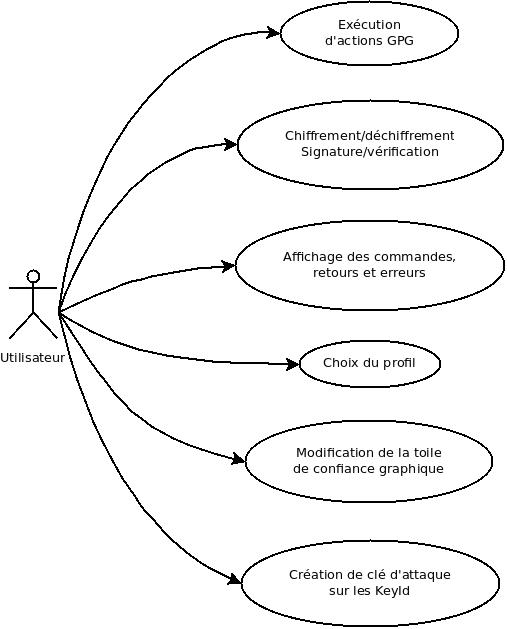
\includegraphics[scale=0.8]{../res/graphics/Diag_utilisations}
 \caption{Diagramme d'utilisation}
\end{figure}

%Cas d'utilisation
\subsection{Interface graphique}

\subsubsection{Cas d'utilisation 1}
\ficheGraphic
% Nom du cas d'utilisation
{Exécution d'actions GPG}
% Acteurs concernés
{Utilisateur}
% Description
{
  Fonctionnement du système pour chaque action nécessitant l'intervention de GPG.
  Toutes ces actions sont spécifiées dans les
  \newline
  \href{http://tools.ietf.org/html/rfc4880}{RFC 4880}
  et \href{http://tools.ietf.org/html/rfc2440}{RFC 2440}
}
% Préconditions
{}
% Evénements déclenchants
{Demande d'action GPG}
% Conditions d'arrêt
{Action terminée}
% Diagramme
{0.5}{../res/graphics/Diag_Seq_Actions_GPG_v3}
% Flots d'exceptions
{Abandon de l'utilisateur.}
% Fin de la fiche du cas d'utilisation 1.
\vspace{0.5cm}

\subsubsection{Cas d'utilisation 2}
\ficheGraphic
% Nom du cas d'utilisation
{Chiffrer/déchiffrer/Signer/Vérifier}
% Acteurs concernés
{Utilisateur}
% Description
{Chiffrer ou déchiffrer ou signer ou vérifier un message copié dans l'éditeur de l'interface.}
% Préconditions
{
  Il y existe plusieurs préconditions :
  \begin{itemize}
    \item Pour déchiffrer ou signer, l'utilisateur possède sa clé privée.
    \item Pour chiffrer, l'utilisateur possède la clé publique du destinataire.
    \item Pour vérifier, l'utilisateur possède la clé publique de l'émetteur.
  \end{itemize}
}
% Evénements déclenchants
{Demande de chiffrement, déchiffrement, signature ou vérification.}
% Conditions d'arrêt
{}
% Diagramme
{0.5}{../res/graphics/Diag_Seq_Chiff_Dechiff_v2}
% Flots d'exceptions
{Abandon de l'utilisateur.}
% Fin de la fiche du cas d'utilisation 2.
\vspace{0.5cm}

Le cadre optionnel permet, lors d'une signature détachée, à l'utilisateur de pouvoir préciser le fichier pour la signature.

L'affichage sortie comporte les informations des retours GPG, tels que le destinataire, l'UI de celui qui a signé, la date, etc., ainsi que le texte une fois chiffré, déchiffré, signé ou vérifié.

\subsubsection{Cas d'utilisation 3}
\ficheGraphic
% Nom du cas d'utilisation
{Affichage des commandes, des retours et des erreurs GPG}
% Acteurs concernés
{Utilisateur}
% Description
{L'utilisateur peut choisir d'afficher ou non les commandes, les retours et les erreurs, associées à chaque action GPG. L'affichage des commandes et l'affichage des retours/erreurs peuvent être activés séparément.}
% Préconditions
{}
% Evénements déclenchants
{Demande de modification de l'affichage.}
% Conditions d'arrêt
{}
% Diagramme
{0.5}{../res/graphics/Diag_Seq_Affichage_Commandes_v2}
% Flots d'exceptions
{Aucun.}   
% Fin de la fiche du cas d'utilisation 3.
\vspace{0.5cm}

Seul l'affichage de la dernière action doit être consultable, c'est-à-dire toutes les commandes GPG, et/ou leurs retours et les erreurs, qui lui sont relatives.

\`{A} tout moment, les informations relatives à la dernière action doivent être consultables par activation de l'affichage des commandes et l'affichage des retours/erreurs, même si ces derniers n'étaient pas activés.


\subsubsection{Cas d'utilisation 4}
\ficheGraphic
% Nom du cas d'utilisation
{Choix du profil utilisateur}
% Acteurs concernés
{Utilisateur}
% Description
{L'utilisateur peut choisir son profil au lancement de l'interface via l'option \texttt{-P}, ou en cours d'utilisation. Si au lancement l'option \texttt{-P} n'est pas précisée, et qu'aucun profil par défaut n'est défini, l'utilisateur doit choisir un profil. Lors de l'installation, un profil par défaut est créé.}
% Préconditions
{Un fichier de configuration de l'interface doit contenir les différents profils, ainsi que l'éventuel profil par défaut. 
Chaque profil possède un trousseau de clé qui lui est propre.}
% Evénements déclenchants
{Ouverture avec option spécifiée, ouverture sans profil par défaut, ou changement de profil en cours d'utilisation.}
% Conditions d'arrêt
{Profil chargé}
% Diagramme
{0.5}{../res/graphics/Diag_Seq_Config}
% Flots d'exceptions
{Abandon de l'utilisateur.}
% Fin de la fiche du cas d'utilisation 4.
\vspace{0.5cm}


\subsubsection{Cas d'utilisation 5}
\ficheGraphic
% Nom du cas d'utilisation
{Modification de la toile de confiance graphique}         
% Acteurs concernés
{Utilisateur}
% Description
{Modification de la Toile de confiance, par un changement de niveau de confiance, l'ajout d'une nouvelle clé ou la modification d'une clé, via la représentation graphique de la toile.}
% Préconditions
{La représentation de la toile de confiance doit apparaître à l'écran.}
% Evénements déclenchants
{Demande de modifications par l'utilisateur.}
% Conditions d'arrêt
{Sauvegarde et mise à jour de l'affichage terminées.}
% Diagramme
{0.5}{../res/graphics/Diag_Seq_Toile}
% Flots d'exceptions
{Abandon de l'utilisateur.}                      
% Fin de la fiche du cas d'utilisation 5.
\vspace{0.5cm}
  

\subsection{Calcul d'une seconde pré-image pour une clé donnée}
  
\subsubsection{Cas d'utilisation 6}
\ficheGraphic
% Nom du cas d'utilisation
{Calcul d'une seconde pré-image pour une clé donnée}
% Acteurs concernés
{Utilisateur}
% Description
{Calcul d'une seconde pré-image sur 4 octets, selon la méthode décrite dans le numéro 75 du MISC, dans l'article à propos de l'attaque sur les KeyId.}
% Préconditions
{Fixer une clé.}
% Evénements déclenchants
{Lancement du calcul.}
% Conditions d'arrêt
{Seconde pré-image trouvée.}
% Diagramme
{0.5}{../res/graphics/Diag_Seq_Attaque}
% Flots d'exceptions
{}
% Fin de la fiche du cas d'utilisation 6.
\vspace{0.5cm}


\subsection{Rapport complet de l'étude de GnuPG}

Le rapport doit énumérer la liste complète des commandes GPG et de les illustrer, ainsi que décrire le fonctionnement de GnuPG.


\subsection{Document d'explications et de recommandations à l'utilisation de l'interface graphique}

Le document d'explications et de recommandations doit permettre à un utilisateur novice en PGP d'utiliser facilement les commandes de base de GPG sur l'interface.
De plus, comme un manuel d'utilisation, il doit décrire l'intégralité des fonctionnalités de l'interface, pour permettre à un utilisateur averti en sécurité informatique de comprendre comment effectuer les réglages techniques sur les clefs et mettre en place sa toile de confiance.


\subsection{Document d'analyse des limites cryptographiques de PGP}

Dans le document d'analyse des limites cryptographiques de PGP doivent figurer les attaques connues sur PGP, répertoriées sur des sites web de veille sur la sécurité informatique. Il devra y figurer aussi les conséquences possibles de la diffusion de la toile de confiance sur les serveurs, au travers de la signature des clés.


\newpage

\section{Exigences opérationnelles}

\begin{tabular}{|>{\centering}p{1cm}|>{}p{11,5cm}|>{\centering}p{2cm}|}
  \hline
  \color{white}\cellcolor{blue}\bfseries{Id}&
  \color{white}\cellcolor{blue}\bfseries{Intitulé}&
  \color{white}\cellcolor{blue}\bfseries{Priorité}\\
  \cr
  \hline
  EO\_1&
  Compatibilité GnuPG 2.0.*&
  Indispensable
  \cr
  \hline
  EO\_2&
  Compatibilité GnuPG 1.4.*&
  Secondaire
  \cr
  \hline
  EO\_3&
  Compatibilité GnuPG 2.1.0&
  Secondaire
  \cr
  \hline
  EO\_4&
  Fonctionnement sous KDE 4.* et 5&
  Indispensable
  \cr
  \hline
  EO\_5&
  Fonctionnement sous Gnome 3.*&
  Important
  \cr
  \hline
  EO\_6&
  Fonctionnement sous Windows&
  Secondaire
  \cr
  \hline
  EO\_7&
  Visualisation graphique de la Toile de confiance&
  Indispensable
  \cr
  \hline
  EO\_8&
  Ouverture de deux interfaces avec des profils différents sur une même session&
  Important
  \cr
  \hline
  EO\_9&
  Connexion SSH : Authentification via une clé signée par GPG&
  Secondaire
  \cr
  \hline
  EO\_10&
  Recherche des clés en local&
  Important
  \cr
  \hline
  EO\_11&
  Choix du logiciel comme logiciel par défaut pour PGP&
  Secondaire
  \cr
  \hline
  EO\_12&
  Choix des couleurs pour les niveaux de confiance et de validité&
  Secondaire
  \cr
  \hline
\end{tabular}\\



\section{Exigences opérationnelles d'interface}

Le client n'a aucune exigence opérationnelle d'interface.


\section{Exigences de qualité}

\begin{tabular}{|>{\centering}p{1cm}|>{}p{11,5cm}|>{\centering}p{2cm}|}
  \hline
  \color{white}\cellcolor{blue}\bfseries{Id}&
  \color{white}\cellcolor{blue}\bfseries{Intitulé}&
  \color{white}\cellcolor{blue}\bfseries{Priorité}\\
  \cr
  \hline
  EQ\_1&
  Représentation des niveaux de confiance et de validité par couleurs&
  Indispensable
  \cr
  \hline
  EQ\_2&
  Temps d'exécution pour l'interface : < temps d'exécution GPG + 100 ms&
  Indispensable
  \cr
  \hline
  EQ\_3&
  Interface livrée sous forme de paquet Ubuntu&
  Important
  \cr
  \hline
  EQ\_4&
  Les pass phrases ne sont jamais affichées en clair&
  Indispensable
  \cr
  \hline
\end{tabular}\\

\section{Exigences de réalisation}

Le client souhaite recevoir une première livraison de l'interface permettant la gestion de base des clés, puis une deuxième incluant également la possibilité de chiffrer, déchiffrer, signer et vérifier des fichiers.

%\begin{tabular}{|>{\centering}p{1,5cm}|>{\centering}p{10cm}|>{\centering}p{3cm}|}
%  \hline
%  \color{white}\cellcolor{blue}\bfseries{Id}&
%  \color{white}\cellcolor{blue}\bfseries{Intitulé}&
%  \color{white}\cellcolor{blue}\bfseries{Priorité}\\
%  \cr
%  \hline
%\end{tabular}\\

\end{document}

